\section{Question Oriented Visual Tasks}
\label{sec-reinforcement-learning}
In this section, we introduce how we do visual tasks that are in connection with questions. 




\subsection{Visual Processing}

In our approach, we build a structure which selects sub-tasks to form a policy which is based on queries. For instance, with the input \textit{which is the defending team?}, the system first predicts the corresponding visual action sequence, which are \textit{Human Module}, \textit{Gesture Module}, \textit{Direction Module}, \textit{Soccer Module}, \textit{Color Blob Module}, \textit{Field Part Module} and \textit{Graph Indicator}. Guided by such sequence, the image features are then extracted by operating relevant vision tasks. An overview is shown in Figure~\ref{fig:RLplot}.

\label{sec-visual-processing}
\begin{figure}[h]
\begin{center}
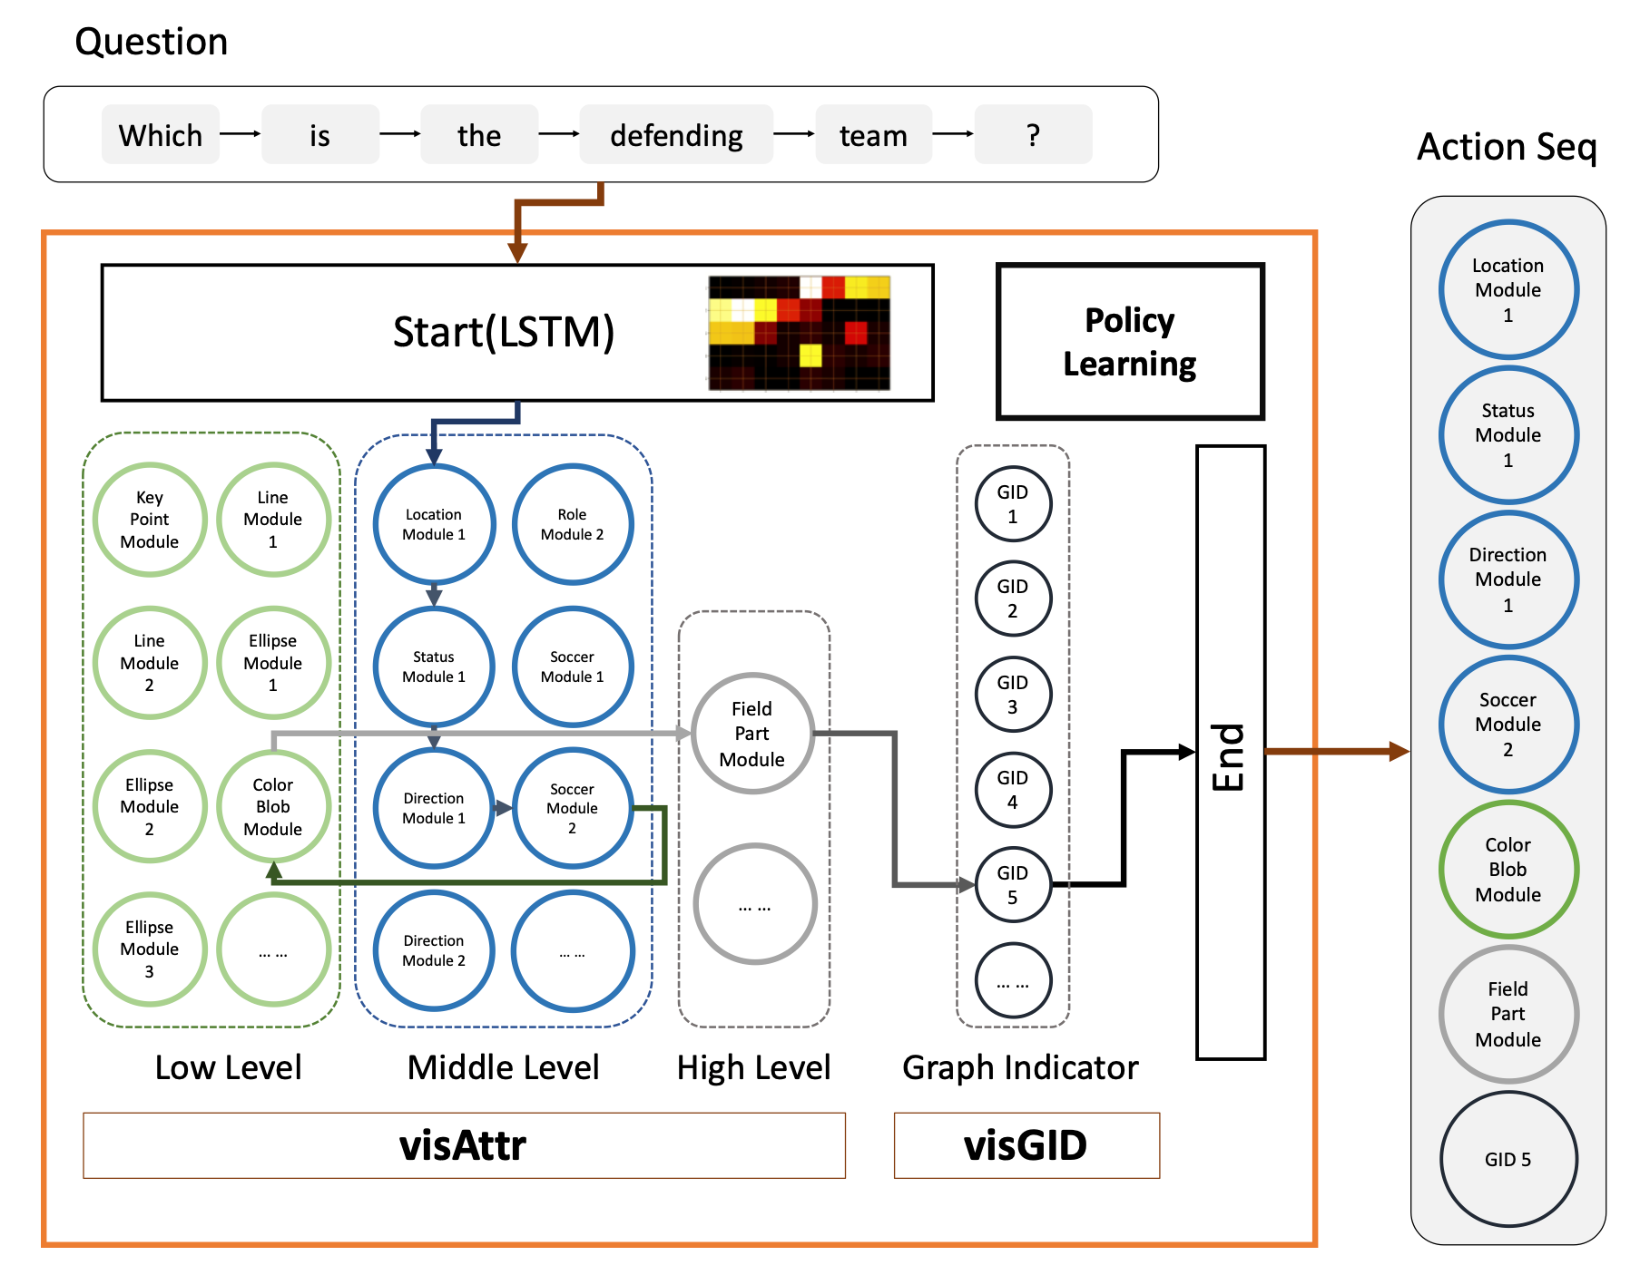
\includegraphics[width=\linewidth]{RLplot.pdf}
\end{center}
\caption{Visual Processing Strategy}
\label{fig:RLplot}
\end{figure}

\subsubsection{Multi-layer LSTM with Attention}
\label{sec-LSTM}
\hspace{\parindent}The task here is to predict the most suitable action modules sequence $\kw{a}$ by given questions $Q$ and preference $pre$. We form the problem of seeking effective answering strategy of question $Q$ and preference $pre$ as a sequence-to-sequence learning problem with attention mechanism. Inspired by~\cite{Bahdanau2016}, we input word feature of questions $w_i^q$, $i\in\|Q\|$ into a LSTM network which is regarded as an encoder and output $h_i$ as the hidden state for $i$th word in the question. By adding soft attention, the context vector $c_i$ is calculated by the following equations.


\begin{small}
\begin{equation} 
    c_i= \sum\nolimits_{j=1}^{\|Q\|} a_{ij}h_{ij}
\end{equation}
\begin{equation} 
    a_{ij}= \frac{exp(e_{ij})}{\sum\nolimits_{k=1}^{\|Q\|} exp(e_{ik})}
\end{equation}
\begin{equation} 
    e_{ij}= a(s_{j-1},h_i)
\end{equation}
\end{small}

\noindent where $h_i$ and $s_j$ are hidden states of encoder and decoder stage, respectively. Here $a_{ij}$ is the attention weights, with higher $a_{ij}$ in $(i, j)$ pair, the more attention will pay in this correlation, thus the $j$th output action $\kw{a}_i$ module will be more influenced by the $i$th input word $w_i^q$ in question. The decode part is similar as traditional recurrent neural networks (RNN). The following steps demonstrates decoding to get the joint distribution of action module sequence $\kw{A} = [\kw{a}_1,\dots,\kw{a}_t]$.

\begin{small}
\begin{equation} 
    p(\kw{A}|Q) = \Pi_{t\in\|\kw{A}\|}~p(\kw{a}_t|\{\kw{a}_1,\dots,\kw{a}_t\},c_i,Q)
\end{equation}
\begin{equation} 
    p(\kw{a}_t|\{\kw{a}_1,\dots,\kw{a}_t\},c_i,Q)= g(\kw{a}_{t-1},s_t,c_i,Q)
\end{equation}
\begin{equation} 
    s_t = f(s_{t-1},\kw{a}_{t-1},c_i)
\end{equation}
\end{small}
\noindent where $g(\cdot)$ is a nonlinear function which outputs the probability of action module \kw{a_{t}}. The probability distribution $p(\kw{A}|Q)$ is used to predict a maximum probability action module sequence by beam search during testing time.

Guided by this action sequence $[\kw{a}_1,\kw{a}_2,\kw{a}_3,\dots,\kw{a}_n]$, actions are selected from the following visual task pool, and comes into next session, visual task selection (\kw{VTS}).


\subsubsection{Visual Task Selection}
\label{sec-VTS}
\hspace{\parindent}\kw{VTS} is guided by the question feature, selecting target visual tasks from the visual task pool by Monte Carlo learning. The task pool is demonstrated in Table~\ref{table:visual_tasks}.


%\begin{table}[th]
%\centering 
%\scriptsize
%
%\begin{tabular}{|l|ll|l|}
%\hline
%visAttr & \multicolumn{1}{l|}{Level}  & Sub-task           & Descriptions                                                                                                                                 \\ \cline{2-4} 
%        & \multicolumn{1}{l|}{Low}    & Keypoint Module    & \multirow{3}{*}{\begin{tabular}[c]{@{}l@{}}To get detailed information of the \\ soccer field $F_{keypoint}$.\end{tabular}}                  \\ \cline{3-3}
%        & \multicolumn{1}{l|}{}       & Line Module        &                                                                                                                                              \\ \cline{3-3}
%        & \multicolumn{1}{l|}{}       & Ellipse Module     &                                                                                                                                              \\ \cline{3-4} 
%        & \multicolumn{1}{l|}{}       & Color Blob Module  & \begin{tabular}[c]{@{}l@{}}To detect blobs of different colors \\ among a region(whole soccer \\ field or a small bounding box).\end{tabular} \\ \cline{2-4} 
%        & \multicolumn{1}{l|}{Middle} & Location Module    & \begin{tabular}[c]{@{}l@{}}To detect the location of the \\ person $P_{location}$.\end{tabular}                                              \\ \cline{3-4} 
%        & \multicolumn{1}{l|}{}       & Status Module      & \begin{tabular}[c]{@{}l@{}}To get the person's gesture \\ $P_{status}$ (standing, moving, \\ expansion).\end{tabular}                        \\ \cline{3-4} 
%        & \multicolumn{1}{l|}{}       & Direction Module   & \begin{tabular}[c]{@{}l@{}}To get whether a person is facing \\ the goal or not $P_{direction}$.\end{tabular}                               \\ \cline{3-4} 
%        & \multicolumn{1}{l|}{}       & Uniform Module     & \begin{tabular}[c]{@{}l@{}}To get the uniform color of the \\ person $P_{uniform}$.\end{tabular}                                              \\ \cline{3-4} 
%        & \multicolumn{1}{l|}{}       & Soccer Module      & \begin{tabular}[c]{@{}l@{}}To detect the location of the \\ soccer $S_{location}$.\end{tabular}                                              \\ \cline{2-4} 
%        & \multicolumn{1}{l|}{High}   & Field Part Module  & \begin{tabular}[c]{@{}l@{}}To detect which part of the\\ soccer field is there in the \\ image $F_{part}$ .\end{tabular}                     \\ \hline
%visGID  &                             & Graph ID Indicator & \begin{tabular}[c]{@{}l@{}}To indicate which type of graph\\ will be used in the following \\process.
%\end{tabular}                          \\ \hline
%\end{tabular}
%\caption{\color{red}Visual Task Pool}
%\label{table:visual_tasks}
%\end{table}

%==========Table===================
\begin{table}[htbp]
	\centering 
	\scriptsize
%\begin{tabularx}{c| c| l | p{3cm} }
\begin{tabularx}{\linewidth}{ c | c| l | X }
	\Xhline{1pt}

%visAttr:
	\multirow{12}{*}[-5em]{visAttr} & {Level}  & Sub-task           & Descriptions                                                                                                                                 \\ \Xcline{2-4}{0.7pt}
	
	% first part
	& \multirow{4}{*}[-12pt]{Low} & Keypoint Module &  \multirow{3}{*}{ \parbox{3cm}{To get detailed information of the soccer field $F_\text{keypoint}$.} }  \\ \cline{3-3}
	& 					& Line Module   & \\\cline{3-3}
	& 					& Ellipse Module    & \\\cline{3-4}
	&					& Color Blob Module & {To detect blobs of different colors  among a region ( whole soccer field or a small bounding box).}\\ \cline{2-4}
	
	% second part
	& \multirow{5}{*}[-28pt]{Middle} & Location Module &  {To detect the location of the person $P_\text{location}$.}\\ \cline{3-4}
	&						  & Status Module   &   {To get the person's gesture  $P_\text{status}$ (standing, moving, expansion).} \\ \cline{3-4}
	&						  & Direction Module   &   {To get whether a person is facing the goal or not $P_\text{direction}$.} \\ \cline{3-4}
	&						  & Uniform Module    &   {To get the uniform color of the person $P_\text{uniform}$.} \\ \cline{3-4}
	&						  & Soccer Module  &  {To detect the location of the soccer $S_\text{location}$.}  \\ \cline{2-4}
	
	% third part
	& \multirow{1}{*}[-4pt]{High} & Field Part Module &  {To detect which part of the soccer field is there in the image $F_\text{part}$.} \\ \hline 
	
%visGID part
\multirow{1}{*}[-8pt]{visGID}  & \multicolumn{2}{c|}{\multirow{1}{*}[-8pt]{Graph ID Indicator}}	 &  {To indicate which type of graph  will be used in the following process.} \\
\Xhline{1pt}
\end{tabularx}
\caption{\color{red}Visual Task Pool}
\label{table:visual_tasks}
\end{table}
%==========Table===================

The pool is constructed by two parts, the first one is \textit{visAttr} which aims to discover the attribute of people, soccer, field and scene~\cite{peixi2019}, while the other one \textit{visGId} is an indicator showing the current question belongs to which graph type. There are three levels of \textit{visAttr}: low, middle and high, which represents different difficulty degree of the vision tasks. 

\begin{figure}[thb]
\centering
        \begin{subfigure}[b]{0.088\textwidth}
                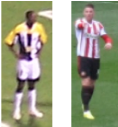
\includegraphics[width=\linewidth]{stand1.png}
                \caption{Standing}
                \label{fig:gull}
        \end{subfigure}\quad
        \begin{subfigure}[b]{0.127\textwidth}
                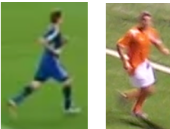
\includegraphics[width=\linewidth]{move1.png}
                \caption{Moving}
                \label{fig:gull2}
        \end{subfigure}\quad
        \begin{subfigure}[b]{0.166\textwidth}
                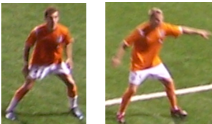
\includegraphics[width=\linewidth]{expand1.png}
                \caption{Expansion}
                \label{fig:tiger}
        \end{subfigure}
        \caption{Person status.}\label{fig:Person Status}
\end{figure}

For each vision task, the approach is not fixed, one task can be achieved by different methods with variance in time and accuracy. For instance, object detection based methods, like Faster R-CNN~\cite{Ren:2015:FRT:2969239.2969250}, R-FCN~\cite{DBLP:conf/nips/DaiLHS16}, SSD~\cite{DBLP:conf/eccv/LiuAESRFB16} or skeleton keypoints detection based method like~\cite{cao2017realtime} and~\cite{wei2016cpm} can be implemented as a set of status module methods, because all of them is able to localize and distinguish people who are moving, standing or with an expansion gesture (Figure~\ref{fig:Person Status}). Thus, the system is not only able to determine whether resembles a vision task module into action module sequence $[\kw{a}_1,\kw{a}_2,\kw{a}_3,\dots,\kw{a}_n]$, it can also select one specific approach under a vision task module, based on question and preference. For the preference, it is clarified in the next section.


\subsubsection{Time and Accuracy Term}
\label{sec-TimeAcc}
\hspace{\parindent} To better balance the accuracy and inference time for a given application, we proposed time and accuracy terms in loss function during training process.

\begin{small}
\begin{equation} 
    L_{\tau\alpha}(\theta) = \ell(\theta,\kw{A}|I, Q) + \gamma\sum_{i\in\|\kw{A}\|}\alpha(\kw{a_i}) + (1-\gamma)\sum_{i\in\|\kw{A}\|}\tau(\kw{a_i})
\end{equation}
\end{small}

\noindent where $\tau(\cdot)$ and $\alpha(\cdot)$represent the pre-tested inference time and inference accuracy, action module sequence \kw{A} samples from joint distribution $p(\kw{A}|Q)$, and here $\ell(\cdot)$ is the softmax loss over the predict score. For the preference term $\gamma$, it ranges from 0 to 1, which represents the preference over time and accuracy.

\subsubsection{Monte Carlo Methods}
\label{sec-MC}
\hspace{\parindent} The task now becomes a policy learning problem. Given a question and preference, output a policy containing a sequence of actions $[\kw{a}_1,\kw{a}_2,\kw{a}_3,\dots,\kw{a}_n]$. There is no ground truth for each steps, but only a final reward indicates that whether the prediction result is correct based on current policy. We involve the concept of Monte Carlo Methods to learn the policy which guides the vision tasks, and such policy network requires an extra reward value in loss.

\begin{small}
\begin{equation} 
    L_{policy}(\theta) = \sum\nolimits_{i\in\|A\|} log\pi(\kw{a}_{i}|Q,\theta)\ell(Q,\kw{A})
\end{equation}
\end{small}

\noindent where \kw{a_{i}} is the action will take, based on current status. $\pi(\cdot)$ is the policy function that maps status to actions, here, the policy is the probability of outputing next action module $\kw{a_{i}}$ based on current status. And $\ell(\cdot)$ here is the softmax loss based on the whole action module sequence $[\kw{a}_1,\kw{a}_2,\kw{a}_3,\dots,\kw{a}_n]$. Since all actions are discrete, which leads to non-differentiable, and back-propagation cannot be used. Policy gradient~\cite{Liu_2017_ICCV} is used here during training. The object function now becomes the combination of policy gradient loss $L_{policy}(\theta)$ with the time-accuracy-balanced loss $L_{\tau\alpha}$, and optimize it by backpropagation for $L_{\tau\alpha}$, while policy gradient for $L_{policy}(\theta)$.


\subsection{Construction of \kw{EAG}}
\label{sec-eag-construction}

After objects that are related to questions are identified, we construct a graph structure, denoted as \kw{EAG}, along the same line as~\cite{peixi2019}. 


\begin{example}
\label{exm-x1}
{\color{red} ADD AN EXAMPLE TO ILLUSTRATE PROGRESS IF NECESSARY!}
\end{example}
